%%%%%%%%%%%%%%%%%%%%%%%%%%%%%%%%%%%%%%%%%%%%%%%%%%%%%%%%%%%%%%%%%%%%%%%%%%
%%%%%                         CHAPITRE 6                            %%%%%%
%%%%%%%%%%%%%%%%%%%%%%%%%%%%%%%%%%%%%%%%%%%%%%%%%%%%%%%%%%%%%%%%%%%%%%%%%%

\lhead[\fancyplain{}{\leftmark}]%Pour les pages paires \bfseries
      {\fancyplain{}{}} %Pour les pages impaires
\chead[\fancyplain{}{}]%
      {\fancyplain{}{}}
\rhead[\fancyplain{}{}]%Pour les pages paires 
      {\fancyplain{}{\rightmark}}%Pour les pages impaires \bfseries
\lfoot[\fancyplain{}{}]%
      {\fancyplain{}{}}
\cfoot[\fancyplain{}{\thepage}]%\bfseries
      {\fancyplain{}{\thepage}} %\bfseries
\rfoot[\fancyplain{}{}]%
     {\fancyplain{}{\scriptsize}}


%%%%%%%%%%%%%%%%%%%%%%%%%%%%%%%%%%%%%%%%%%%%%%%%%%%%%%%%%%%%%%%%%%%%%%%%%%
%%%%%                      Start part here                          %%%%%%
%%%%%%%%%%%%%%%%%%%%%%%%%%%%%%%%%%%%%%%%%%%%%%%%%%%%%%%%%%%%%%%%%%%%%%%%%%

\chapter{Application to boxing, using action cameras}
\label{ch:6}

%==============================================================================	Résumé du chapitre

\begin{center}
\rule{0.7\linewidth}{.5pt}
\begin{minipage}{0.7\linewidth}
\smallskip

\textit{Boxing is a challenging sport for motion analysis, because movements are fast, 3 dimensional, and involves the whole body. Moreover, it is usually not possible to equip a boxer with markers, lightning conditions and large capture volumes make the classic marker-based difficult, research-grade cameras are too cumbersome to set up in a timely way and lower-end cameras can't be synchronized by hardware, nor with a flash in the context of a competition.\newline\newline
The objective of the study was to verify whether it is possible to accurately measure Key Performance Indicators (KPIs) in boxing, with a markerless protocol and under suboptimal conditions. This was concurrently validated with a marker-based protocol. A secondary goal was to compare the impact on result quality of a markerless analysis with post-calibration and post-synchronization, to the impact of choosing a different 2D pose estimation model. We conclude that KPIs are remarkably well evaluated in all conditions, although the choice of the 2D pose estimator is more influential than the protocol. \newline \newline
This chapter is adapted from the poster presented at the congress of the European College of Sport Science (ECSS): "A 3D markerless protocol with action cameras – Key performance indicators in boxing" \cite{Pagnon2022c}.
}

%\smallskip
\end{minipage}
\smallskip
\rule{0.7\linewidth}{.5pt}
\end{center}

\clearpage

\minitoc

\vspace*{3cm}

\begin{figure}[hbtp]
	\centering
	\def\svgwidth{1\columnwidth}
	\fontsize{10pt}{10pt}\selectfont
	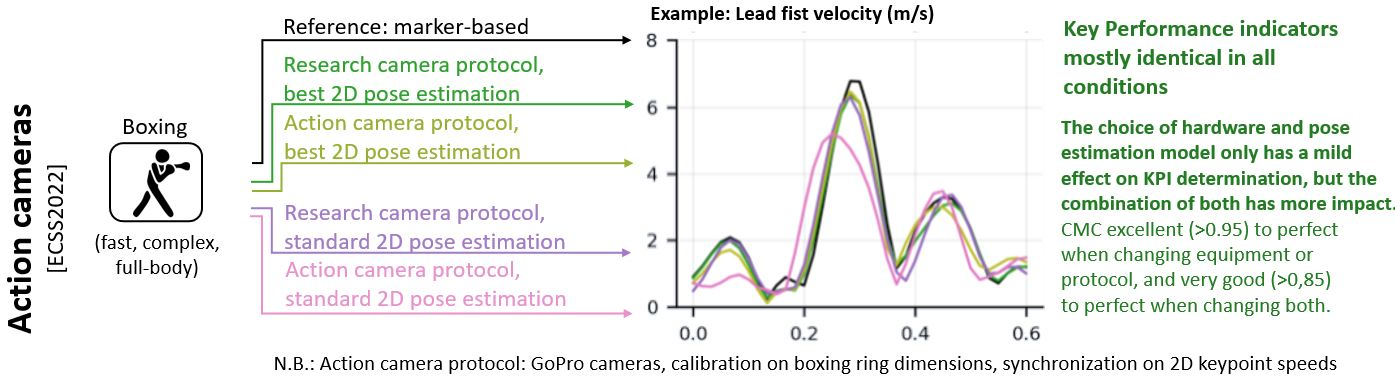
\includegraphics[width=\linewidth]{"../Intro/Figures/Fig_VisAbstract4.JPG"}
      \caption{Visual abstract for the assessment of KPIs in boxing with Pose2Sim \cite{Pagnon2022c}.}
	\label{fig_visabstract4}
\end{figure}

\newpage






\section{Objectives}

\subsection{Key Performance Indicators in boxing}

Key Performance Indicators (KPIs) are a set of variables which need to be measured in priority, in order to assess performance, or to evaluate main areas where work is needed. Although they are more known in the fields of management or of the industry, identifying them is also important in sports \cite{Butterworth2013}. Determining them would typically be done with Principal Component Analysis (PCA) \cite{Hotelling1933}, which helps to find the main over a large amount of measurable variables, for example in tennis \cite{ODonoghue2008}. However, this might lead to the selection of indicators which may be hard to retrieve, or not intuitively meaningful (for example, if they consist in the combination of some seemingly unrelated variables.) Moreover, coaches usually have a very fine and comprehensive understanding of what to look for in their sport. As a consequence, another way of determining KPIs is to simply ask them for guidance, and verifying which then to run correlation analysis. 



eigenvectors, helps grouping data together


cf anthropometric arm length


and they are the ones who will use the results of the analysis. Therefore, it is important to involve them in the process of identifying the KPIs, and to make sure that they are meaningful for them.

oftentimes already know what they need to measure, and they have a very fine view of the 

come up to the same conclusions as coaches have, decades ago



In boxing, the analysis of the kinematics of the upper body is of particular interest, because it is the main source of power in punches. The main objective of this study was to evaluate the accuracy of the 3D kinematic analysis of the upper body in boxing, using a markerless protocol and action cameras. The secondary objective was to compare the impact on result quality of a markerless analysis with post-calibration and post-synchronization, to the impact of choosing a different 2D pose estimation model.


However, the kinematics of some sports is less impredictive (marathon running vs. boxing)

Kinematic analysis in sports helps improve sports technique, prevent injuries, and reveal different motor skills among athletes. 


In boxing, punching speed is of uttermost importance. However, it is not generated in the same way in jabs (mostly translational movement) as in hooks (mostly rotational). Key performance indicators (KPIs) have been determined [1], but they are usually investigated with subjective visual observation. 

shadow boxing




\subsection{Limits of research-grade systems in competitions}

When finer analysis is needed, marker-based kinematics is usually employed. 

However, what if:

•Wearing markers is not conceivable? 

•Research-grade cameras are not available?

•Classic marker-based calibration is impossible? 

•Usual synchronization methods are not feasible? 

Subsidiary question: Does the choice of the 2D pose estimation model matter?



Markers, Cameras et setup, Calibration, synchronization, Feedback



% Calibration remains a challenging task in daylight, at a distance, with non research-grade cameras, and in a sports scene. It could be useful to make it more robust, either by implementing the Aniposelib library \cite{Karashchuk2020}, or by calibrating automatically on people’s limb length \cite{Liu2022a}.

% La calibration sera impossible si vous êtes trop loin. Les marqueurs réfléchissants ne réfléchiront pas la lumière des caméras (à tester : marqueurs actifs).  
% Si vous voulez effectuer une post-calibration avec un checkerboard (avec cette méthode par exemple), il faudra que le checkerboard soit assez grand pour qu’il soit bien détecté. Une règle simple : pour avoir de bons résultats, la largeur du checkerboard doit remplir au moins un cinquième de l’image. Si vous voulez couvrir une scène de 20 m, il faudra un checkerboard de 4 m de large...  
% Autre solution non testée : Calculer hors manip les paramètres intrinsèques des caméras vidéo. En manip, placer côte à côte des caméras MoCap Arqus et vidéo Miqus, faire la calibration des Arqus (plus performantes), et ajouter une translation dans les paramètres extrinsèques des Arqus pour avoir ceux des Miqus. 


% Adding muscles which were stripped from the skeleton in the OpenSim model could allow for joint kinetics prediction. Neural networks could be trained to estimate ground reaction forces from kinetics on specific tasks, without the use of a force platform [Oh2013, Johnson2018, Mundt2019].
% Using Xsens markers hidden by clothes in Kinovis? Although not gold-standard


\subsection{Objectives}

Concurrently validating the accuracy of KPI measurements in boxing with suboptimal markerless protocols.


\section{Methods}
\subsection{4 conditions}
\blindtext

\subsection{Pose-calibration on ring dimensions}
\blindtext

\subsection{Post-synchronization on 2D movement speeds}
\blindtext

\subsection{GoPro spatio-temporal base into Qualysis'}
\blindtext

\subsection{Statistical analysis}
\blindtext


\section{Results}
\blindtext


\section{Discussion}
\subsection{Equipment and protocol vs. pose estimation model}
\blindtext

\subsection{Pros and cons of different systems}

Auto-calibration with person?

Cloud computing?

Temporal consistency?

Shape information for less cameras?

Rolling shutter: Pour les GoPros, la fréquence de roll du shutter de haut en bas est approxivement la même que la fréquence d'acquisition, donc vu qu'on peut filmer jusqu'à 240 Hz en full HD, 120Hz en 4K, et 60Hz à 5.3k, je doute que ce soit un vrai problème...
Pas de retour visuel instantanné
Synchro : nouvelles avec GPS, sinon méthodes
Calib : Mieux qu'avec Qualisys en plein air

\blindtext
